\chapter{Probability Spaces, Random Variables and Distribution Fuunctions}

\begin{definition}[Random variable]
Let $(\Omega, \F, \Prob)$ be a probability space.  A measurable function $X: \Omega\mapsto \Re$ is called a random variable. The law of the random variable is the probability measure $\mu$ on $(\Re, \B )$ defined by
\begin{equation}
\mu(A)=\Prob(X\in A), A\in\B.
\end{equation}
The distribution function of $X$ is defined by
\begin{equation}
F(x)=\mu((-\infty, x])=\Prob(X\leq x)
\end{equation}
for real $x$.
\end{definition}


\begin{notes}
\begin{enumerate}
\item $\Prob(\Omega)=1$ and $X^{-1}(B)\in \F$ for any $B\in\B$ implies that $\Prob(X^{-1}(B))$ makes sense. This is the law of the random variable $X$
\item $B=(-\infty, x]$ is the Borel set. $F(x)$ is a probability distribution
\end{enumerate}
\end{notes}



\begin{theorem}\label{thm:prob:1}
Let $F$  be a distribution function of some random variable $X$. Then
\begin{enumerate}
\item $F(x)\leq F(y)$ whenever $x\leq y$,
\item $\lim\limits_{x\to -\infty} F(x)=0$, $\lim\limits_{x\to+\infty}F(x)=1$,
\item $F$ is right-continuous
\end{enumerate}
\end{theorem}


Recall the standard normal distribution

\begin{equation*}
\phi(x) = \frac{1}{2\pi}e^{-x^2/2}, \qquad -\infty <x < \infty
\end{equation*}
The distribution function of the standard normal distribution is right continuous. Another example is the Poisson distribution. Refer to Figure \ref{fig:1}.


\begin{figure}[h]
\caption{\label{fig:1} Graph of the Poisson cdf with $\lambda=1$, $\lambda=2$, and $\lambda=4$. Source: \url{https://en.wikipedia.org/wiki/Poisson_distribution}}
\centering
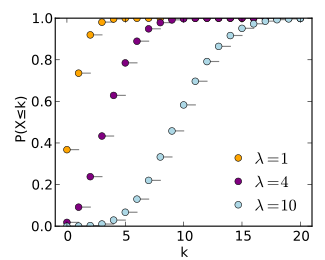
\includegraphics[width=0.4\linewidth]{figures/Poisson_cdf.png}
\end{figure}



We now prove Theorem \ref{thm:prob:1}.

\begin{proof}
\begin{prooflist}
\item If $x\leq y$ then $(-\infty, x]\subseteq (-\infty, y]$ and it follows that $F(x)=\mu((-\infty,x])\leq \mu((-\infty, y])=F(y)$.
\item Get the intersections of the intervals $r\in \bigcup\limits_{n=1}^{\infty}(-\infty,-n]$. (See Fig. \ref{fig:prob:2}) That is, $r\leq -n$ for all $n$.

\begin{figure}[h]
\caption{\label{fig:prob:2} Intervals $(-\infty,-n]$}
\centering
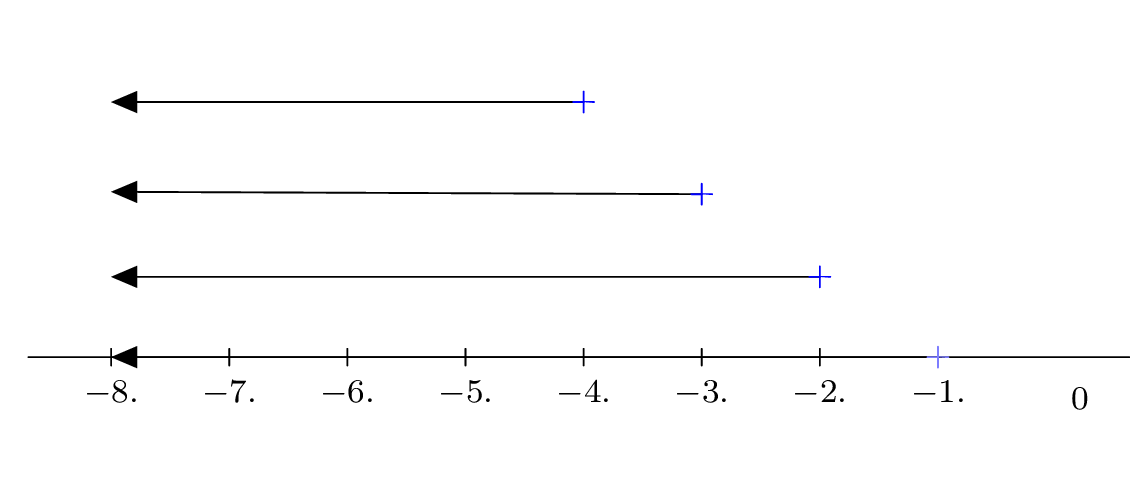
\includegraphics[width=0.75\linewidth]{figures/overlap-intervals.png}
\end{figure}
Note that $\bigcap\limits_{n=1}^\infty (-\infty, -n]=\varnothing$ so that
\begin{align*}
\lim_{x\to\-\infty}F(x)&=\lim_{n\to\infty}F(-n)=\lim_{n\to\infty}\mu((-\infty,-n])\\
	&=\mu\left(\bigcap_{n=1}^\infty(-\infty,-n]\right)\qquad (decreasing)\\
	&=\mu(\varnothing)=0
\end{align*}
Similarly,
\begin{align*}
\bigcup_{n=1}^\infty (-\infty,n]=\Re
\end{align*}
and
\begin{align*}
\lim\limits_{x\to+\infty}F(x)=\mu\left(\bigcup_{n=1}^\infty (-\infty,n]\right)=1
\end{align*}


\item For right continuity\footnote{Remember from calculus that right continuity means $\lim\limits_{y\to x^+}F(y)=F(x)$}, note that
\begin{equation*}
\lim\limits_{n\to\infty}F\left(x+\frac{1}{n}\right)=\mu\left(\bigcap_{n=1}^\infty\left(-\infty,x+\frac{1}{n}\right]\right)=F(x)
\end{equation*}
To see this, not that
\begin{align*}
\lim\limits_{n\to\infty}F\left(x+\frac{1}{n}\right)&=
	\lim\limits_{n\to\infty}\mu\left(\left(-\infty, x+\frac{1}{n}\right]\right)\\
	&=\mu\left(\bigcap_{n=1}^\infty\left(-\infty,x+\frac{1}{n}\right]\right)
\end{align*}
If $y\in\left(-\infty,x+\frac{1}{n}\right]$ for all $n$, then $y\leq x$. To see this, if $y>x$ then if $x+1>y>x$ then there is an $m$ such tht $y>x+\frac{1}{m}>x$ contradicting the original assumption. So if $y\leq x+\frac{1}{n}$ for all $n$, then $y\leq x$. Therefore,
\begin{align*}
\lim\limits_{n\to\infty}F\left(x+\frac{1}{n}\right)&=\mu\left(\bigcap_{n=1}^\infty\left(-\infty,x+\frac{1}{n}\right]\right)\\
	&=\mu((-\infty,x])\\
	&=F(x)
\end{align*}
\end{prooflist}
\end{proof}


Is the converse of Theorem \ref{thm:prob:1} true? To prove this, we need to find $x$ and show that $F$ is really its distribution function. This is the content of the next theorem.


\begin{theorem}
If $F$ is a nondecreasing, right-continuous function with $\lim\limits_{x\to-\infty}F(x)=0$ and $\lim\limits_{x\to+\infty}F(x)=1$, then there exists on some probability space a random variable $X$ for which $F(x)=\Prob(X\leq x)$.
\end{theorem}

\begin{proof}
Define the random variable $X$ on $([0,1], \B[0,1], \lambda)$ by $X(\omega)=\inf\{z:F(z)\geq \omega \}$. Now, if $z>X(\omega)$ then $F(z)\geq \omega$, so by right-continuity, $F(X(\omega))\geq \omega$. If, in addition $X(\omega)\leq c$ then $\omega\leq F(X(\omega))\leq F(c)$. Thus $\omega\leq F(c)$ if and only if $X(\omega)\leq c$, so that $\Prob(X\leq c)=\lambda([0,F(c)])=F(c)$.
\end{proof}



\begin{proof}
Define the random variable $X$ on $([0,1], B[0,1], \lambda)$, (where $\lambda$ is Lebesque measure) by $X(\omega)=\inf\{z: F(z)\geq \omega \}$. Now, if $z>X(\omega)$ then $F(z)>\omega$ so by right-continuity, $F(X(\omega))\geq \omega$. If, in addition, $X(\omega)\leq c$, then $F(X(\omega))\leq F(c)$. Thus $\omega\leq F(c)$ if and only if $X(\omega)\leq c$ so that $\Prob(X\leq c)=\lambda([0,F(c)])=F(c)$.


Now, whenever $z> X(\omega)$, $F(z)\geq \omega$. Thus $\lim\limits_{z\to X(\omega)^+} F(z)\geq\omega$. But since $F(z)$ is right-continuous, we have $\lim\limits_{z\to X(\omega^+)} F(z)\geq\omega$


So $\Prob(X(\omega)\leq c)=\Prob(X\leq c)$. Note that $\Prob(X\leq c)=\lambda(\{\omega: \omega\leq F(c) \})=\lambda([0,F(c)])=F(c)$.
\end{proof}

The foregoing theory shows that we don't need to know about the probability space as long as we know the distribution. that is why we an talk about a normal distribution without knowing the space of concern.